\documentclass{article}

\usepackage[utf8]{inputenc}
\usepackage[T1]{fontenc}
\usepackage{lipsum}
\usepackage{graphicx}
\usepackage{amsmath}
\usepackage[margin=1in]{geometry}
\usepackage{titlesec}
\usepackage{enumitem}

\titleformat{\section} 
{\LARGE\bfseries}{\thesection}{1em}{}

\titleformat{\subsection} 
{\Large\bfseries}{\thesection}{1em}{}

\begin{document}

\pagestyle{empty}

\section*{Diagramma Entità Relazione} 
\large

Il modello \textbf{entità-relazione} è un modello per la \textbf{rappresentazione concettuale} dei dati ad alto livello di astrazione. Si basa su una rappresentazione grafica, attraverso \textbf{diagrammi}. Si tratta di un modello utile per modellare i dati di interesse di un database e per la sua documentazione. E' indipendente dal modello logico in uso e dal DBMS di riferimento.\\
Si osservino ora i diversi componenti di un diagramma \textit{entità-relazione}.

\subsection*{Entità}
\large

Un'\textbf{entità} è una classe di oggetti della realtà di interesse con proprietà comuni e con esistenza autonoma. Graficamente un'entità viene rappresentata attraverso un \textbf{rettangolo}.
\begin{center}
    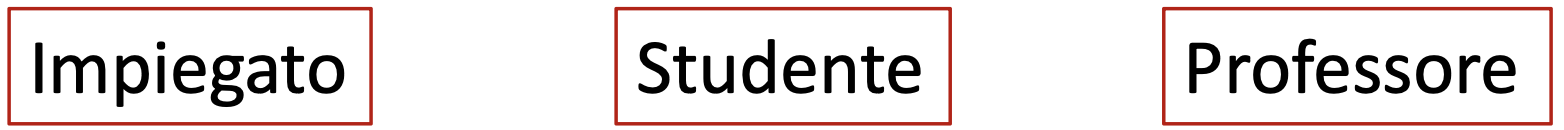
\includegraphics[width=0.55\textwidth]{foto 1.png}
\end{center}
Un'\textbf{entità può essere tradotta in una tabella} del modello relazionale, di cui però non è ancora definito lo schema. Ad ogni entità è associato un \textbf{nome}, che identifica l'oggetto rappresentato. Per convenzione, si usano \textbf{nomi al singolare} per rappresentare entità.\\
L'\textbf{istanza di un'entità} è uno \textit{specifico oggetto appartenente a quell'entità}.
\begin{center}
    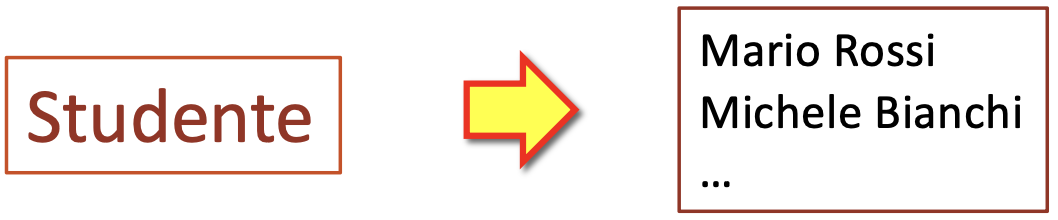
\includegraphics[width=0.4\textwidth]{foto 2.png}
\end{center}

\subsection*{Relazioni}
\large

Una \textbf{relazione} è un legame logico fra due o più entità, rilevante nel sistema che si sta modellando. Graficamente una relazione viene rappresentata attraverso un \textbf{rombo/diamante} collegato ad entità, anche più di due.
\begin{center}
    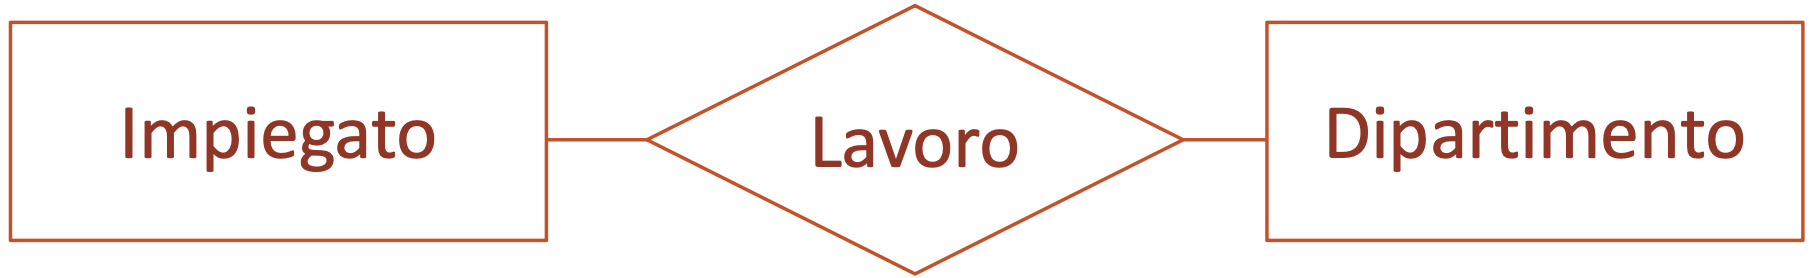
\includegraphics[width=0.5\textwidth]{foto 3.png}
\end{center}
Una \textbf{relazione può essere tradotta in una tabella} del modello relazionale, di cui però non è ancora definito lo schema. Ad ogni relazione è associato un \textbf{nome}, che la identifica nello schema. Per convenzione, si usano \textbf{nomi al singolare} (non verbi se possibile) per rappresentare le relazioni.\\
L'\textbf{istanza di una relazione} è una \textit{combinazione di istante dell'entità} che prendono parte all'associazione.
\begin{center}
    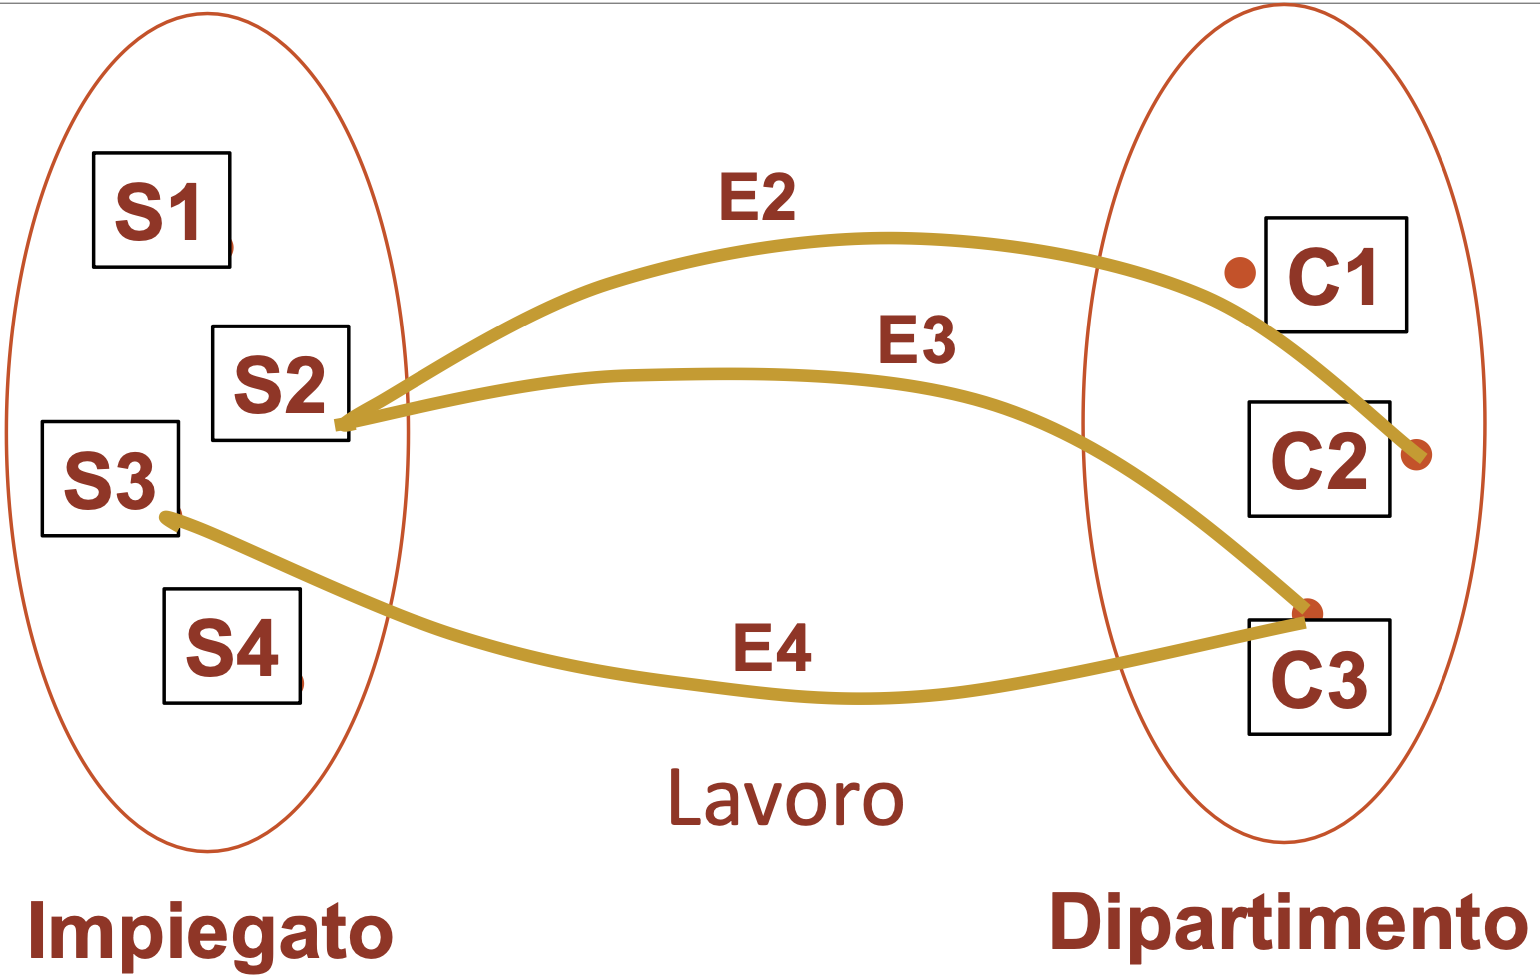
\includegraphics[width=0.45\textwidth]{foto 4.png}
\end{center}
Si osservino ora diversi esempi di \textit{relazioni}:
\begin{itemize}[label={-}, leftmargin=1cm]
    \item \textbf{Relazioni binarie}: 2 entità coinvolte
    \begin{center}
        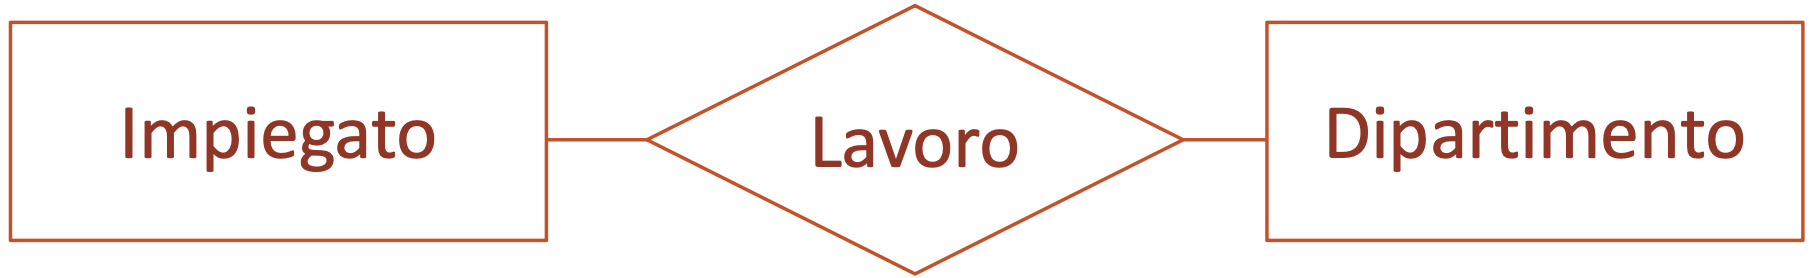
\includegraphics[width=0.45\textwidth]{foto 3.png}
    \end{center}
    \item \textbf{Relazioni n-arie}: numero arbitrario di entità
    \begin{center}
        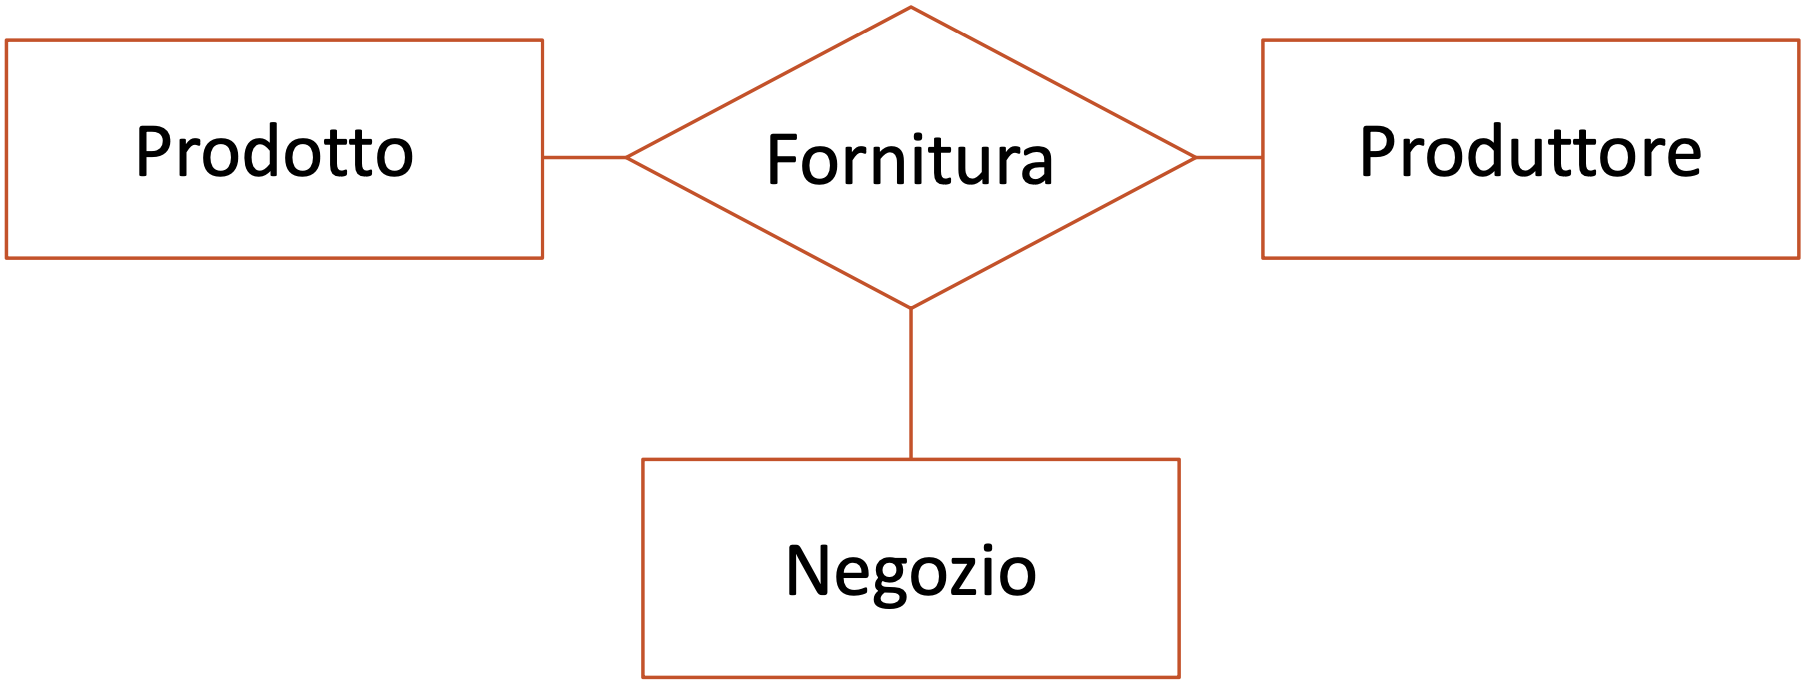
\includegraphics[width=0.45\textwidth]{foto 5.png}
    \end{center}
    \item \textbf{Relazione ricorsiva}: coinvolge più istanze della stessa entità. E' possibile anche definire un \textbf{ruolo} per ciascun ramo della relazione.
    \begin{center}
        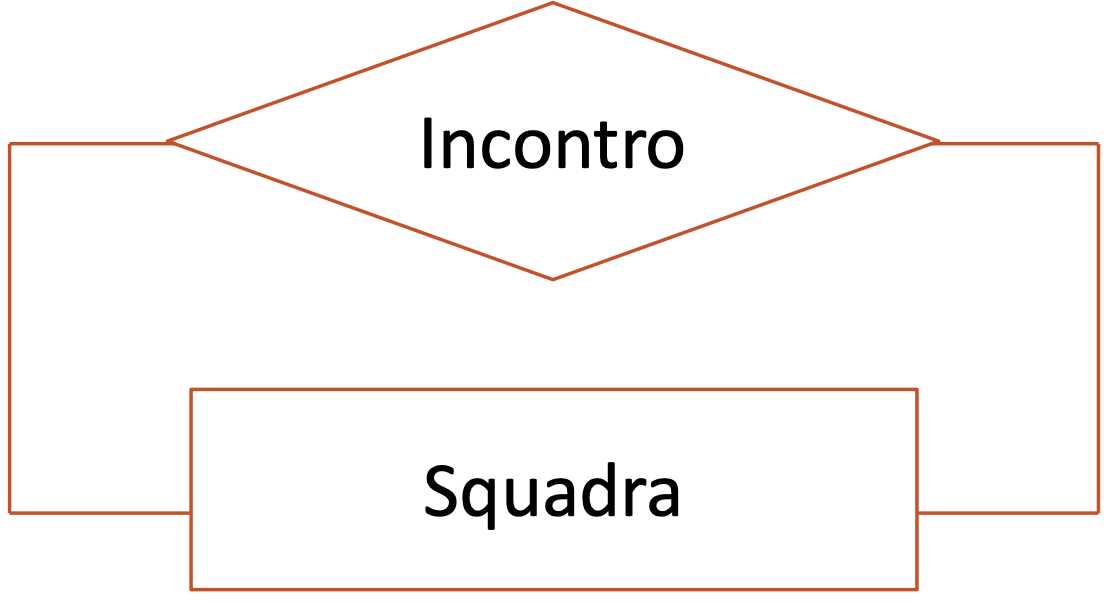
\includegraphics[width=0.35\textwidth]{foto 6.png}
    \end{center}
\end{itemize}

\subsection*{Attributi}
\large

Un \textbf{attributo} è una proprietà elementare di un'entità o di una relazione del modello. Ogni attributo è definito su un dominio specifico.
\begin{center}
    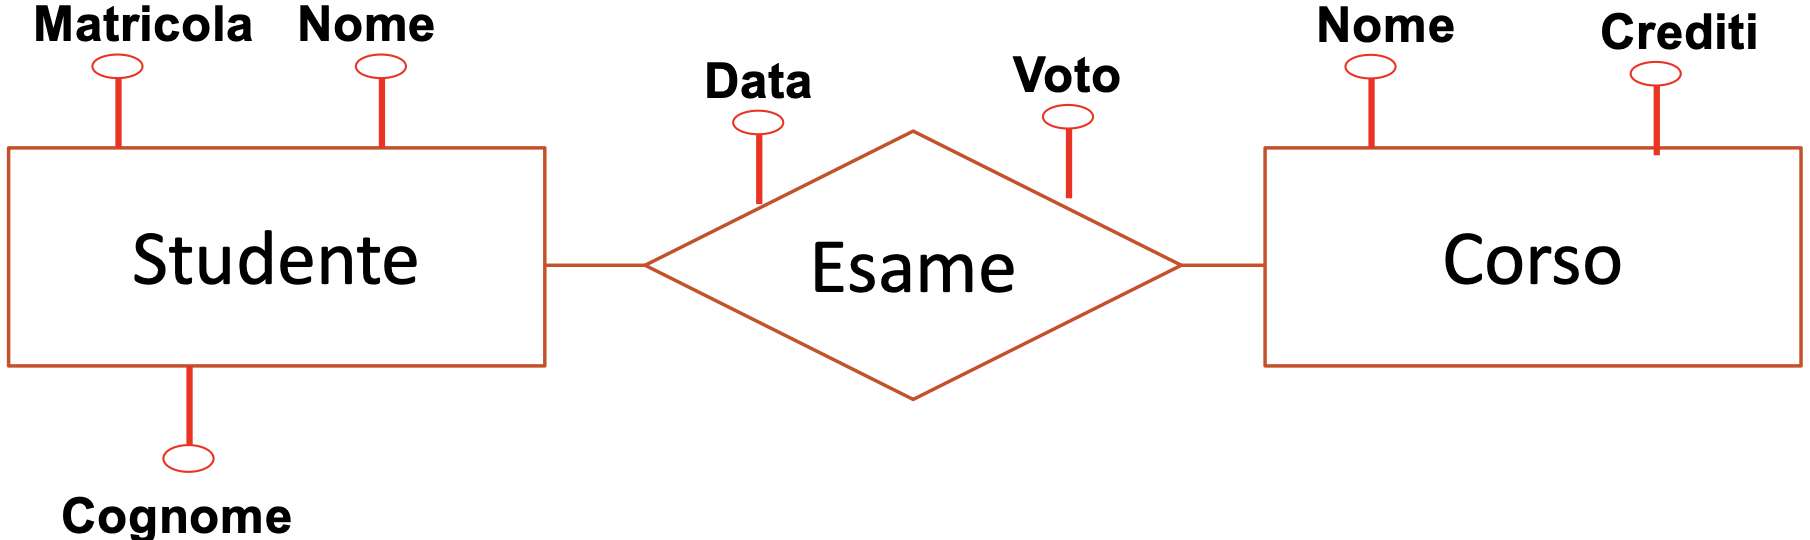
\includegraphics[width=0.5\textwidth]{foto 7.png}
\end{center}
E' possibile definire \textbf{attributi composti} come unione di attributi affini di una certa entità/relazione. Sono rappresentati graficamente da un \textbf{ovale}.
\begin{center}
    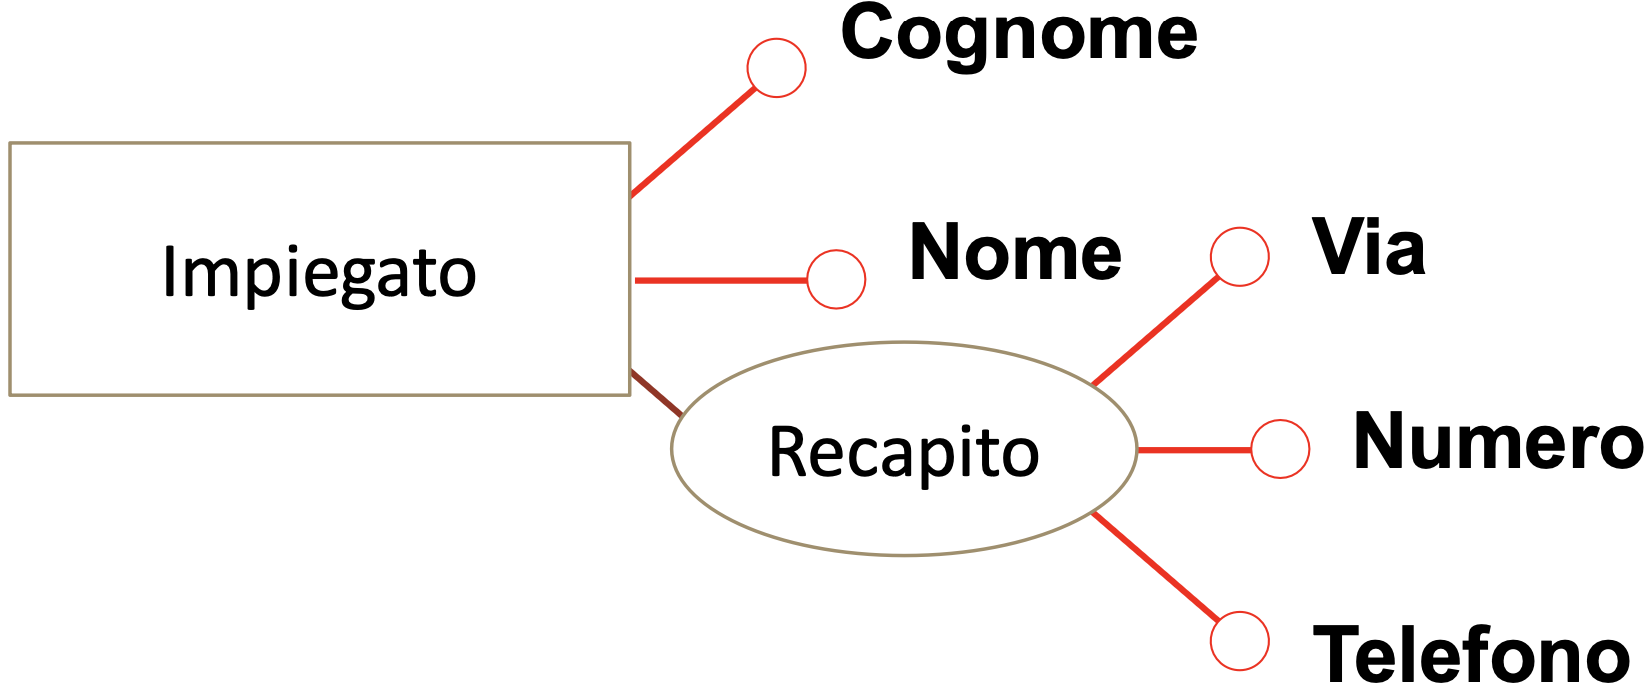
\includegraphics[width=0.5\textwidth]{foto 8.png}\vspace{20pt}\\
\end{center}

\subsection*{Cardinalità delle relazioni}
\large

La \textbf{cardinalità delle relazioni} è una coppia di valori \textbf{(min, max)} che specificano il numero minimo/massimo di occorrenze della relazione cui ogni istanza di entità può partecipare. 
\begin{center}
    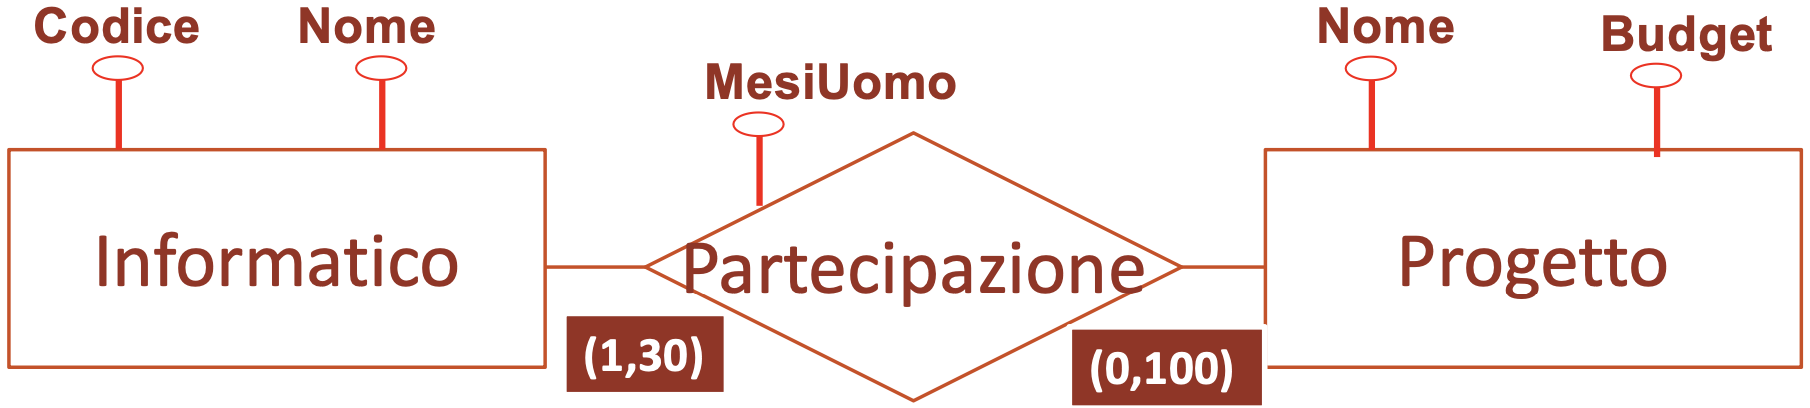
\includegraphics[width=0.5\textwidth]{foto 9.png}
\end{center}
Dato il seguente esempio, si possono notare i seguenti \textit{vincoli}:
\begin{itemize}[label={-}, leftmargin=1cm]
    \item Ogni istanza di \textit{Informatico} deve comparire \textbf{almeno in un'istanza} della relazione \textit{Partecipazione}
    \item La stessa istanza di \textit{Informatico} può comparire \textbf{al massimo in 30 istanze} della relazione \textit{Partecipazione}
    \item La stessa istanza di \textit{Progetto} può comparire \textbf{al massimo in 100 istanze} della relazione \textit{Partecipazione}
\end{itemize}
In generale, nella pratica vengono utilizzati solo \textit{due valori per il minimo}:
\begin{itemize}[label={-}, leftmargin=1cm]
    \item \textbf{0}: partecipazione \textbf{opzionale} dell'entità
    \item \textbf{1}: partecipazione \textbf{obbligatoria} dell'entità
\end{itemize}
Viceversa, nella pratica vengono utilizzati solo \textit{due valori per il massimo}:
\begin{itemize}[label={-}, leftmargin=1cm]
    \item \textbf{1}: al massimo una istanza coinvolta
    \item \textbf{N}: non esiste un limite massimo\\
\end{itemize}
In base al valore della \textbf{cardinalità massima delle entità} \textit{E1} ed \textit{E2} coinvolte in una relazione \textit{R}, si distinguono \textbf{tre casi}:
\begin{itemize}[label={-}, leftmargin=1cm]
    \item Relazioni \textbf{uno ad uno}: \textit{cardMax(E1) = 1}, \textit{cardMax(E2) = 1}
    \item Relazioni \textbf{uno a molti}: \textit{cardMax(E1) = 1}, \textit{cardMax(E2) = N} oppure \textit{cardMax(E1) = N}, \textit{cardMax(E2) = 1}
    \item Relazioni \textbf{molti a molti}: \textit{cardMax(E1) = N}, \textit{cardMax(E2) = N}
\end{itemize}
Il tipo di relazione viene stabilito in base alla \textbf{realtà di interesse}, la quale emerge dal documento di specifica dei dati. Questa informazione è fondamentale in \textbf{fase di traduzione del modello}.\\
\begin{center}
    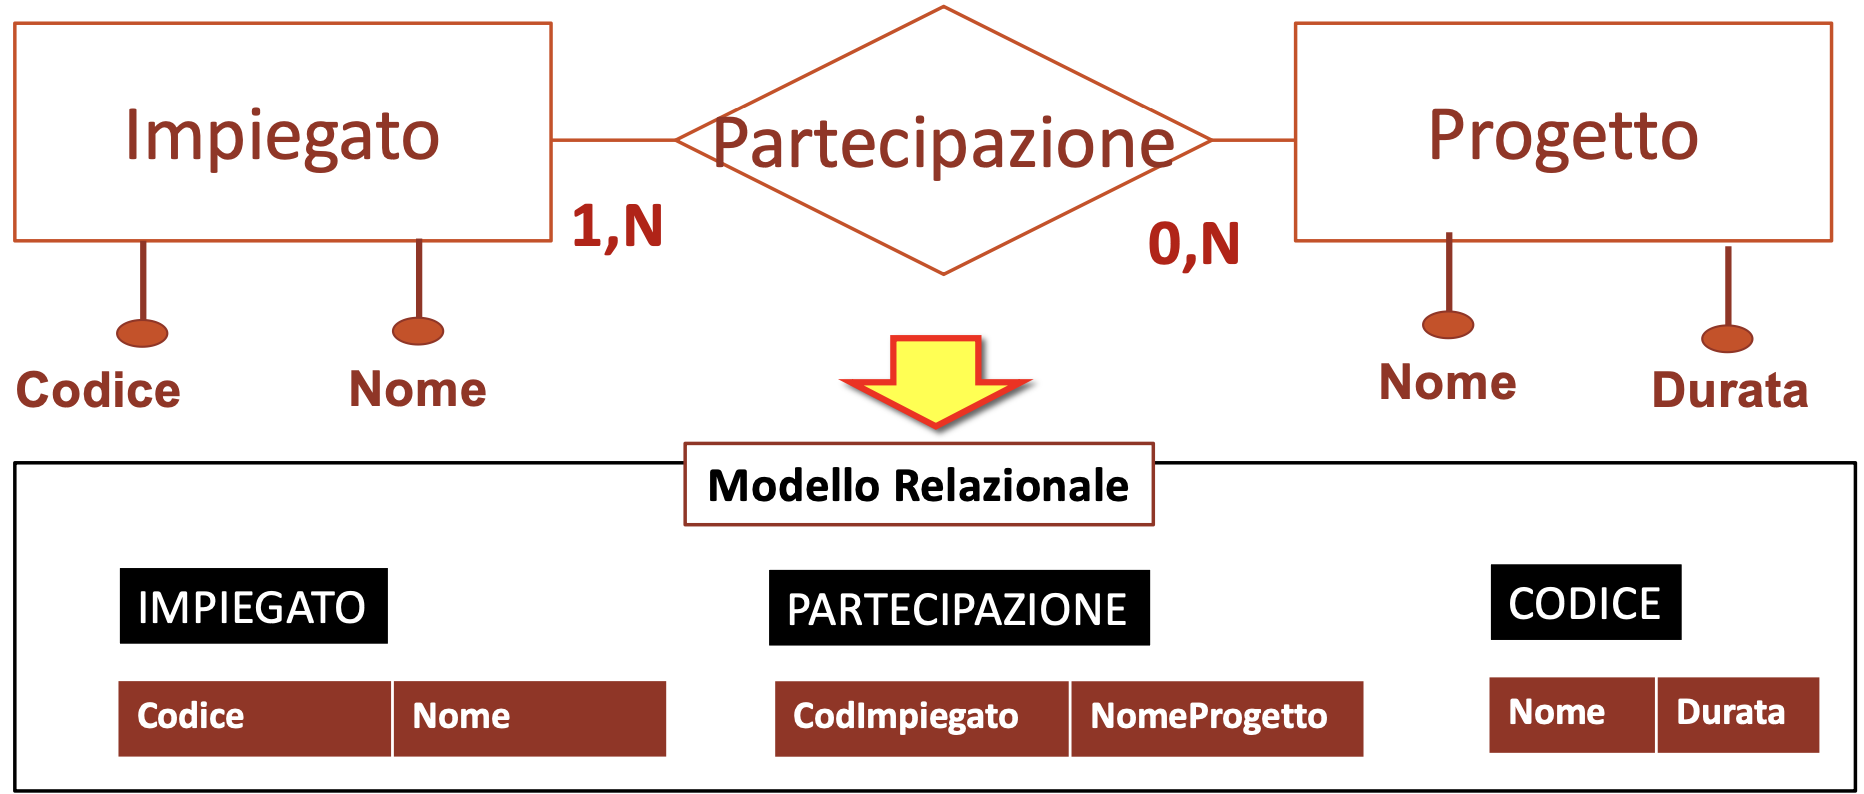
\includegraphics[width=0.6\textwidth]{foto 10.png}
\end{center}
\textit{Nota Bene}: la cardinalità può essere specificata anche in presenza di \textbf{relazioni ricorsive con ruoli}.

\subsection*{Cardinalità degli attributi}
\large

Come per le relazioni, anche per gli \textbf{attributi} è possibile definire una \textbf{cardinalità} minima e massima. La cardinalità è applicabile anche agli \textbf{attributi composti}.
\begin{center}
    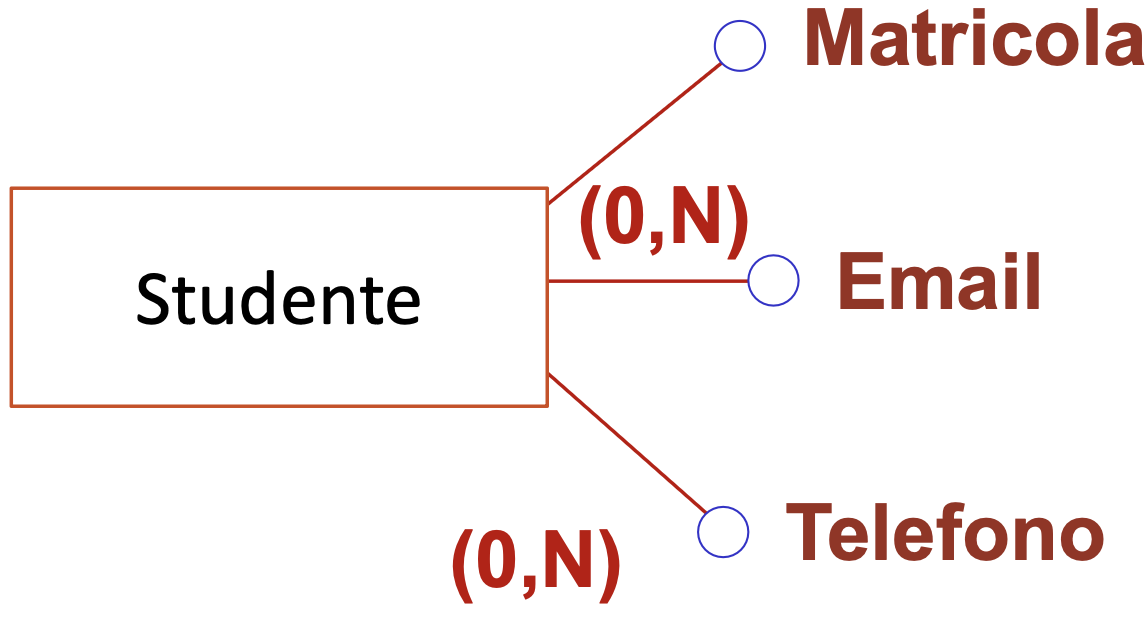
\includegraphics[width=0.4\textwidth]{foto 11.png}
\end{center}

\subsection*{Identificatori}
\large

Un \textbf{identificatore} è uno strumento per identificare in maniera univoca le istanze di una entità. Corrisponde al concetto di \textbf{chiave} nel modello relazionale, per questo motivo deve sottostare al requisito di minimalità.\\
Ogni entità \textbf{deve avere un identificatore}, ma non necessariamente la relazione. Un identificatore può essere:
\begin{itemize}[label={-}, leftmargin=1cm]
    \item \textbf{Interno}: composto da \textit{attributi dell'entità}
    \item \textbf{Esterno}: composto da \textit{attributi dell'entità + entità esterne}\\
\end{itemize}
\textit{Identificatore interno}\\
Un \textbf{identificatore interno} è composto da uno o più attributi dell'entità.
\begin{center}
    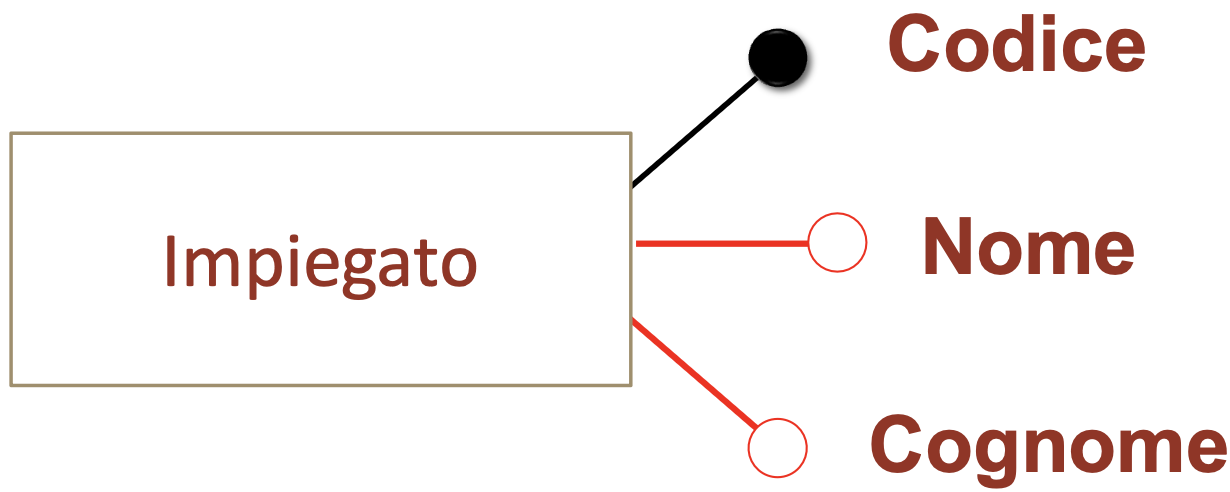
\includegraphics[width=0.4\textwidth]{foto 12.png}
\end{center}
In questo caso, \textit{Codice} è l'identificatore interno. \textbf{Non possono esistere} due istanze di Impiegato con lo \textbf{stesso Codice}.\\
\textit{Nota Bene}: gli attributi che formano l'identificatore interno di un'entità devono avere cardinalità \textbf{(1, 1)}.\vspace{110pt}\\
\textit{Identificatore esterno}\\
Un \textbf{identificatore esterno} include anche entità esterne, collegate attraverso relazioni all'entità corrente.
\begin{center}
    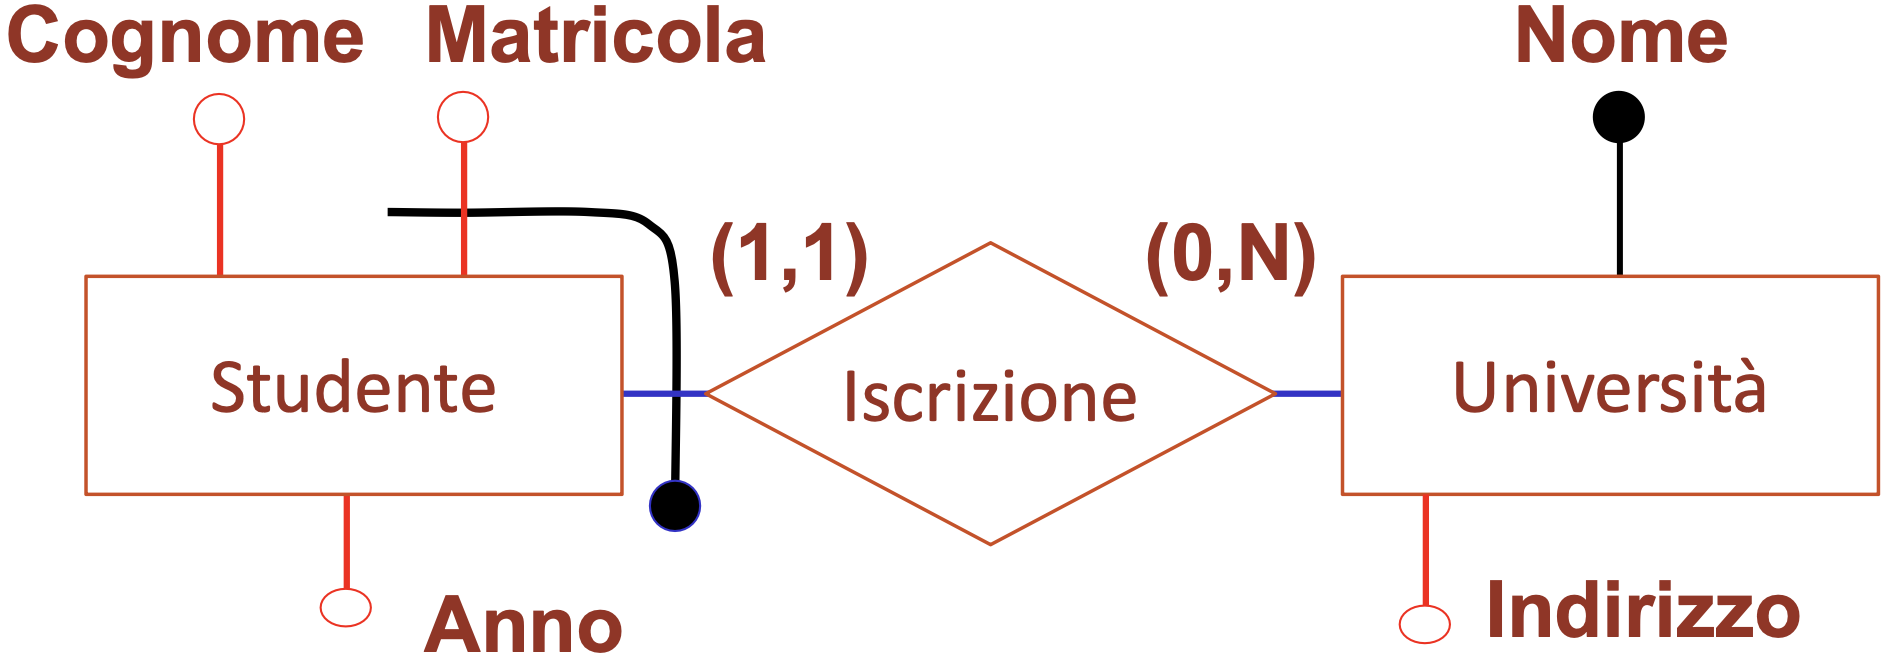
\includegraphics[width=0.6\textwidth]{foto 13.png}
\end{center}
Alcune proprietà dell'\textit{identificatore esterno} sono:
\begin{itemize}[label={-}, leftmargin=1cm]
    \item Può comprendere anche \textbf{attributi} dell'entità corrente
    \item L'entità esterna \textbf{deve essere in relazione (1, 1)} con l'entità corrente
\end{itemize}
In pratica, gli identificatori esterni servono a modellare le situazioni in cui \textbf{un'istanza di un'entità ha valori univoci solo all'interno di un certo contesto}, definito dalle relazioni cui partecipa l'entità.

\subsection*{Generalizzazioni}
\large

Una \textbf{generalizzazione} definisce una gerarchia tra entità basata sul concetto di ereditarietà.
\begin{center}
    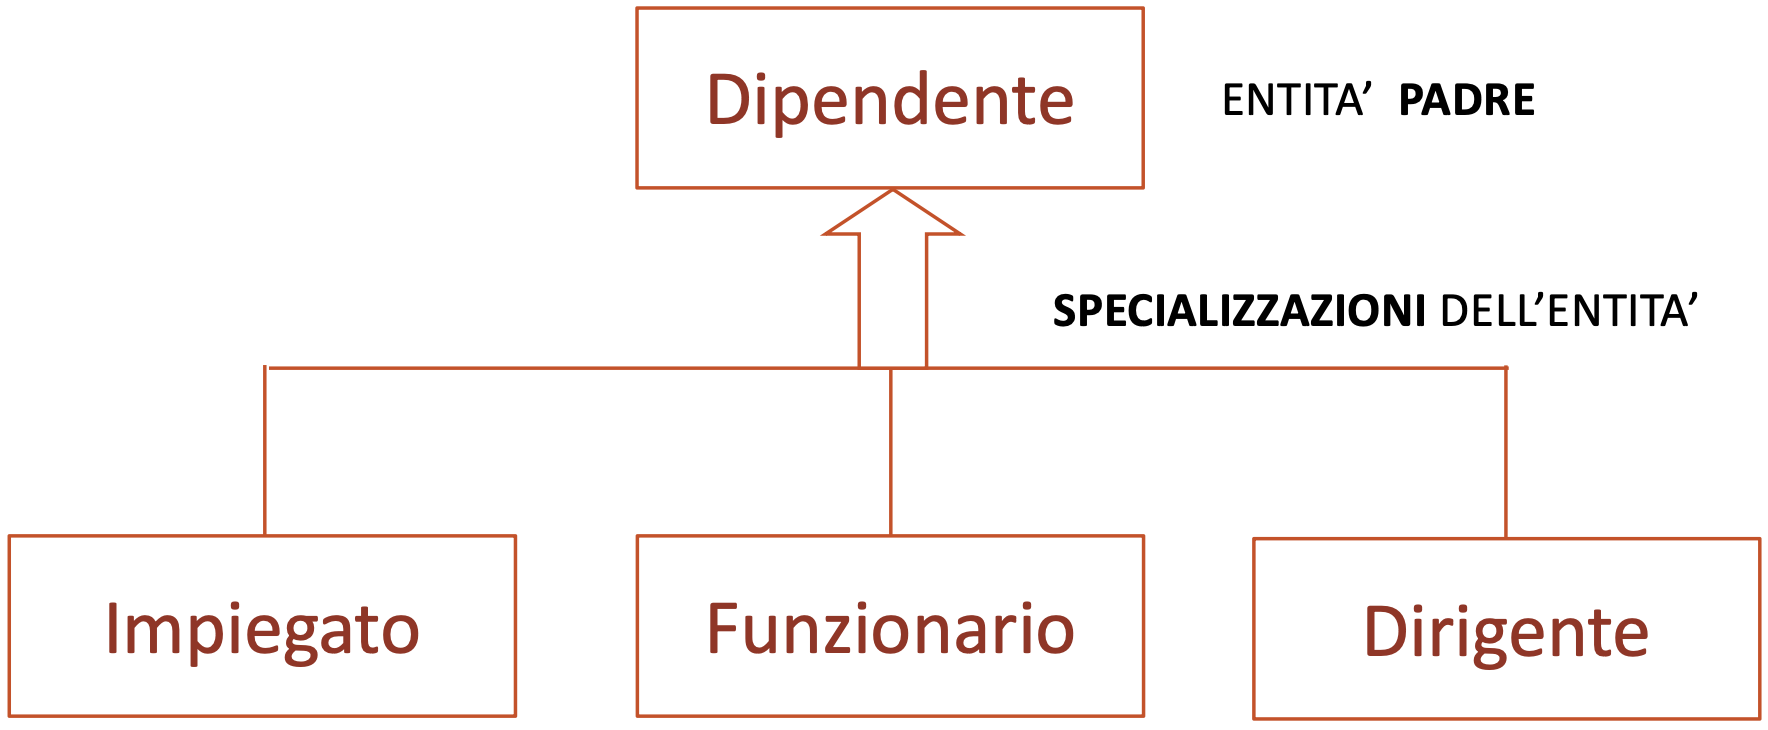
\includegraphics[width=0.6\textwidth]{foto 14.png}
\end{center}
Un'entità \textit{E} è una \textbf{generalizzazione} di \textit{$E_1$, $E_2$, \dots, $E_n$} se ogni istanza di \textit{$E_1$, $E_2$, \dots, $E_n$} lo è anche di \textit{E}. Quindi, \textit{$E_1$, $E_2$, \dots, $E_n$} sono \textbf{specializzazioni} di \textit{E}.\\
Tutti gli attributi di \textit{E} sono \textbf{anche attributi} di \textit{$E_1$, $E_2$, \dots, $E_n$}, e \textbf{partecipano a tutte le relazioni} di \textit{E}.\vspace*{14pt}\\
Possono esistere due tipologie distinte di generalizzazioni:
\begin{itemize}[label={-}, leftmargin=1cm]
    \item \textbf{Generalizzazione parziale}: esistono occorrenze dell'entità padre che non sono occorrenze delle entità figlie
    \item \textbf{Generalizzazione totale}: ogni occorrenza dell'entità padre è occorrenza di almeno una delle due entità figlie\vspace*{20pt}\\
\end{itemize}
Inoltre, è possibile definire \textbf{generalizzazioni a cascata}:
\begin{center}
    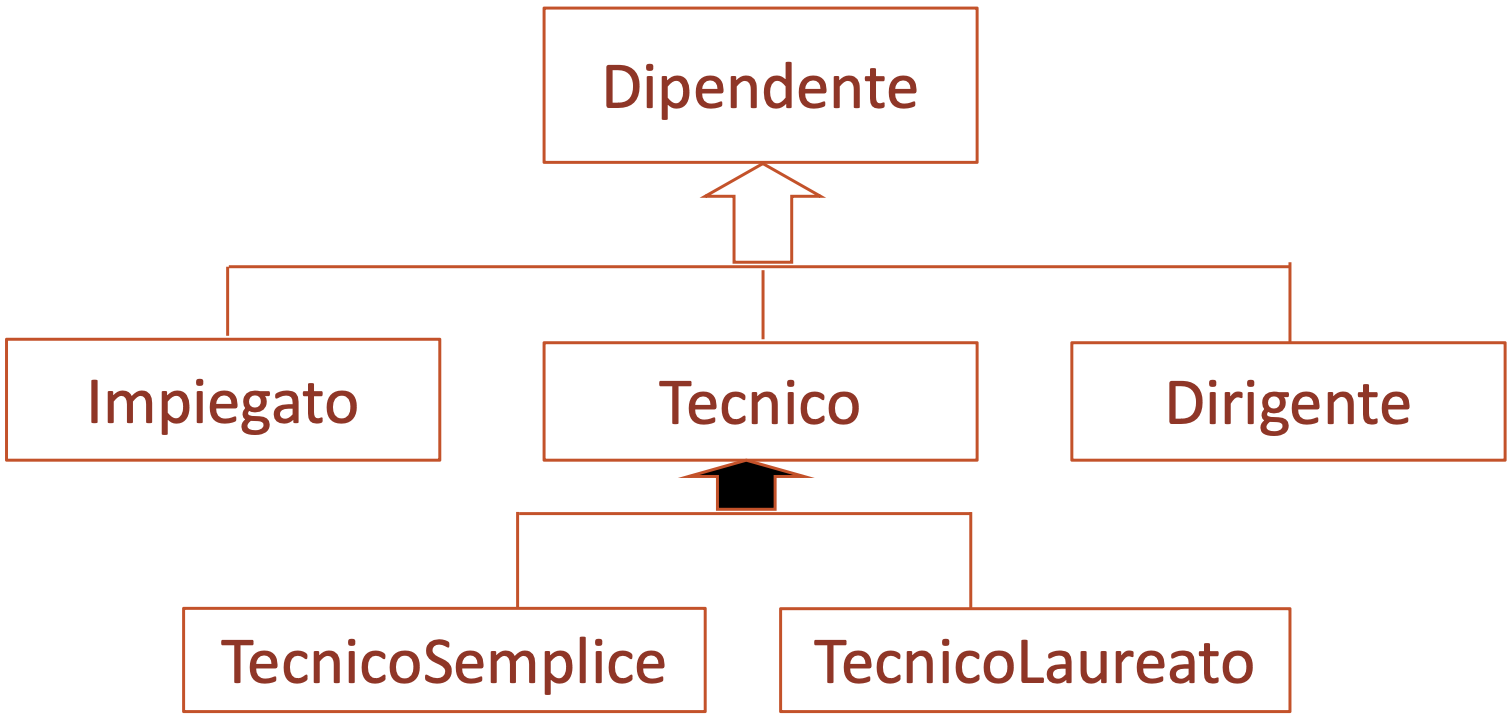
\includegraphics[width=0.6\textwidth]{foto 15.png}\vspace{14pt}\\
\end{center}

\subsection*{Riassunto sintassi generale}
\large

Si osservi ora un riassunto della sintassi generale per la realizzazione di un modello entità relazione:
\begin{itemize}[label={-}, leftmargin=1cm]
    \item \textbf{Entità}
    \begin{center}
        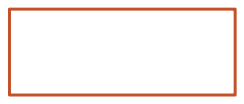
\includegraphics[width=0.15\textwidth]{foto 16.png}
    \end{center}
    \item \textbf{Relazione}:
    \begin{center}
        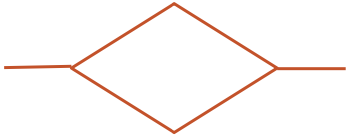
\includegraphics[width=0.15\textwidth]{foto 17.png}
    \end{center}
    \item \textbf{Attributo}:
    \begin{center}
        
\includegraphics[width=0.15\textwidth]{foto 18.png}
    \end{center}
    \item \textbf{Cardinalità delle relazioni}:
    \begin{center}
        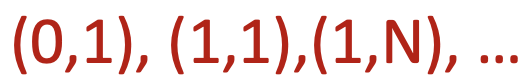
\includegraphics[width=0.15\textwidth]{foto 19.png}
    \end{center}
    \item \textbf{Cardinalità degli attributi}:
    \begin{center}
        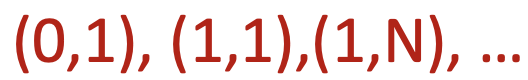
\includegraphics[width=0.15\textwidth]{foto 20.png}
    \end{center}
    \item \textbf{Identificatori}:
    \begin{center}
        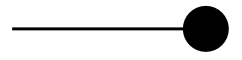
\includegraphics[width=0.15\textwidth]{foto 21.png}
    \end{center}
    \item \textbf{Generalizzazioni}:
    \begin{center}
        
\includegraphics[width=0.15\textwidth]{foto 22.png}\vspace{50pt}\\
    \end{center}
\end{itemize}
Si introduce inoltre il concetto di \textbf{dizionario dei dati}, tabelle contenenti la descrizione delle entità/relazioni del modello E/R. Si osservi un esempio di dizionario delle entità:
\begin{center}
    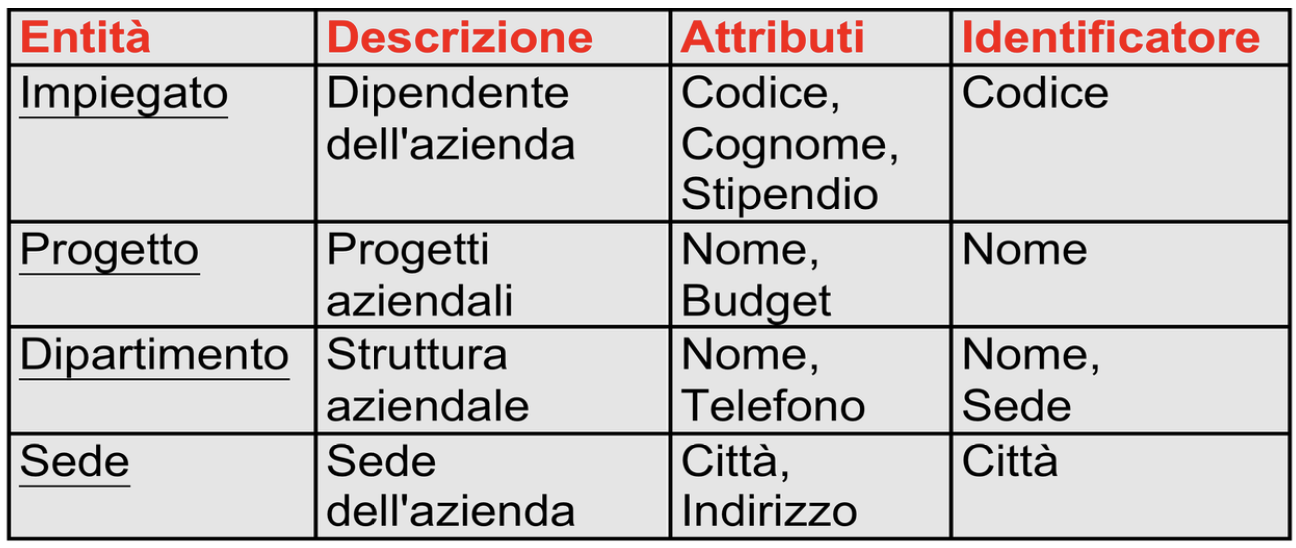
\includegraphics[width=0.6\textwidth]{foto 23.png}
\end{center}
ed uno di dizionario delle relazioni:
\begin{center}
    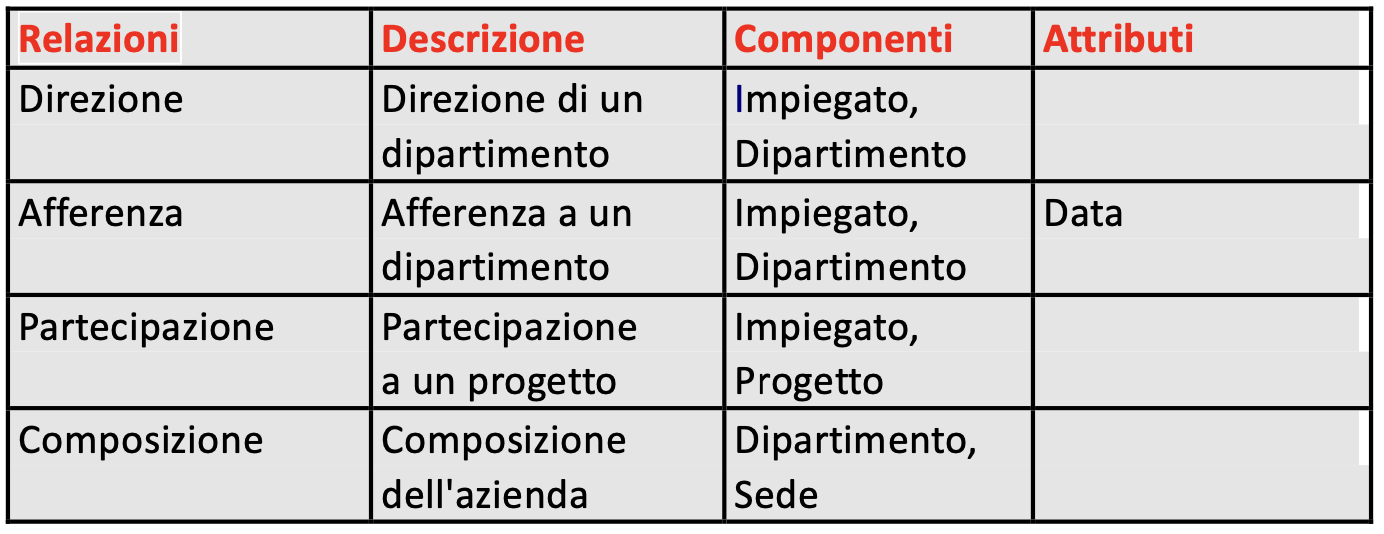
\includegraphics[width=0.6\textwidth]{foto 24.png}\vspace{14pt}\\
\end{center}
Si presenta però un'ultima problematica: il diagramma E/R è uno strumento di modellazione molto potente e generale, ma \textbf{non tutti i vincoli presenti nelle specifiche sono esprimibili nel modello}. Per esprimere i vincoli non rappresentabili dal diagramma E/R, si utilizzano delle \textbf{business rules}, le quali descrivono un concetto rilevante per l'applicazione. Esprimono inoltre i vincoli sui dati dell'applicazione e la derivazione dei differenti concetti presenti.\\
Le business rules possono essere raccolte in \textbf{tabelle}, e devono essere \textbf{allegate al diagramma E/R}. Un esempio può essere:
\begin{center}
    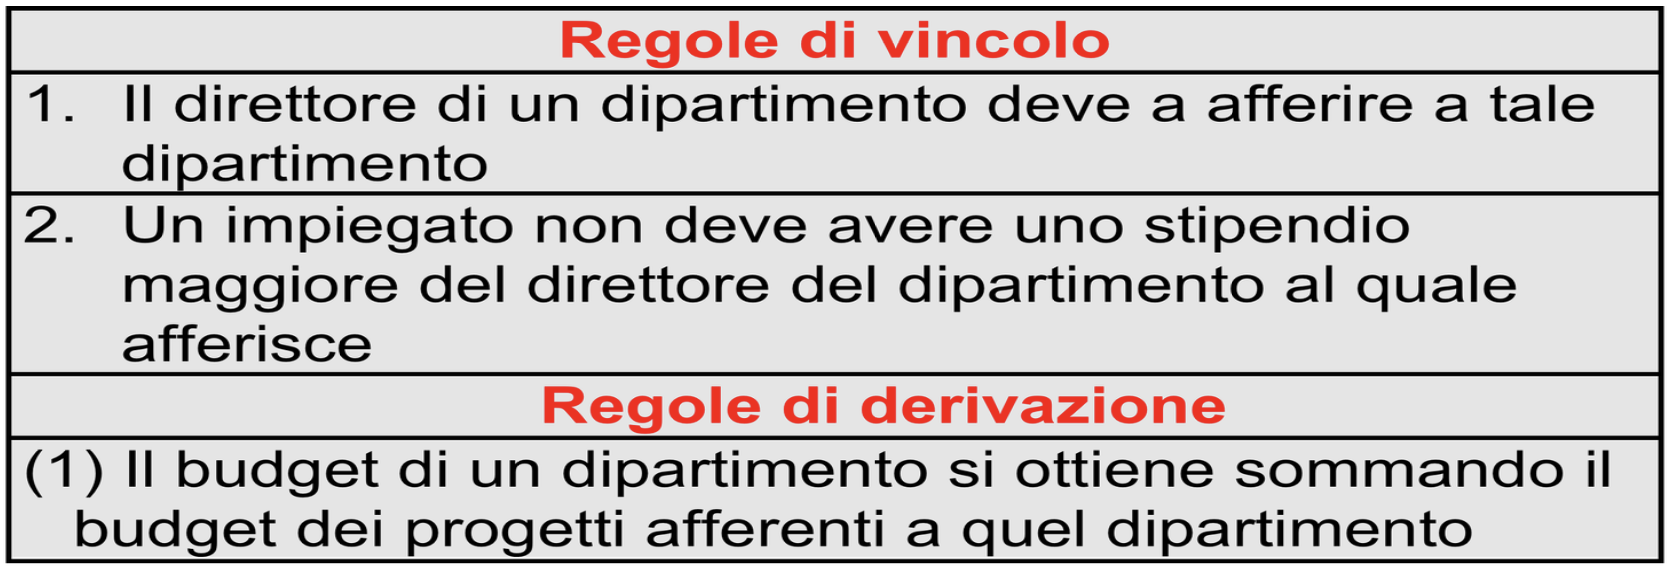
\includegraphics[width=0.6\textwidth]{foto 25.png}
\end{center}
\end{document}